\subsection{UC23 - Prenotazione tavolo}\label{usecase:23}

\begin{figure}[H]
  \centering
  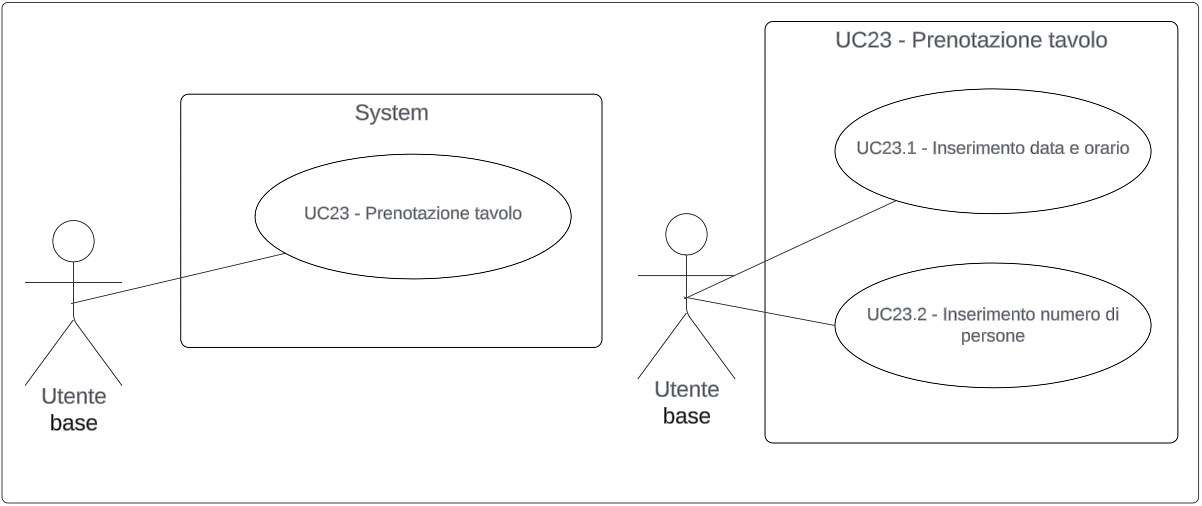
\includegraphics[width=0.9\linewidth]{ucd/UCD23_new.png}
  \caption{Prenotazione tavolo}
\end{figure}

\textbf{Attori principali}:
\begin{itemize}
    \item Utente base.
\end{itemize}
\textbf{Precondizione}:
\begin{itemize}
    \item L'utente base è connesso al $\textit{sistema}_G$.
\end{itemize}
\textbf{Postcondizione}:
\begin{itemize}
    \item L'utente ha richiesto una $\textit{prenotazione}_G$ in un ristorante;
    \item Il $\textit{sistema}_G$ ha inviato una notifica al ristorante selezionato.
\end{itemize}
\textbf{Scenario principale}:
\begin{enumerate}
    \item L'utente ha selezionato il ristorante in cui vuole prenotare;
    \item In fase di $\textit{prenotazione}_G$, l'utente inserisce:
    \begin{itemize}
        \item La data e l'orario di arrivo (\nameref{usecase:23_1});
        \item Il numero di persone (\nameref{usecase:23_2});
        % \item Le altre persone presenti al tavolo con il relativo username/email utente (\nameref{usecase:23_3});
    \end{itemize}
    \item Dopo aver completato l'inserimento di tutte le informazioni richieste, viene generato un link univoco relativo all'$\textit{ordinazione}_G$ collaborativa da condividere con tutti i partecipanti al tavolo. 
    \item Infine, il $\textit{sistema}_G$ invia una notifica di una richiesta di $\textit{prenotazione}_G$ agli amministratori del ristorante selezionato.
\end{enumerate}
\textbf{Scenari alternativi}:
\begin{itemize}
    \item Se si verifica che:
    \begin{enumerate}
        \item L'utente decide di cancellare la $\textit{prenotazione}_G$;
        \item Il ristorante non possiede tavoli liberi con le informazioni selezionate. Allora l'utente visualizza un messaggio di errore;
    \end{enumerate}
    \item La $\textit{prenotazione}_G$ viene cancellata.
\end{itemize}



\subsubsection{UC23.1 - Inserimento data e ora}\label{usecase:23_1}
\textbf{Attori}:
\begin{itemize}
    \item Utente base.
\end{itemize}
\textbf{Precondizioni}:
\begin{itemize}
    \item L'utente base è connesso al $\textit{sistema}_G$.
\end{itemize}
\textbf{Postcondizioni}:
\begin{itemize}
    \item L'utente ha inserito correttamente la data e l'orario di arrivo per la $\textit{prenotazione}_G$.
\end{itemize}
\textbf{Scenario principale}:
\begin{enumerate}
    \item L'utente inserisce la data desiderata per la $\textit{prenotazione}_G$ nel formato appropriato;
    \item L'utente specifica l'orario di arrivo previsto nel formato appropriato.
\end{enumerate}



\subsubsection{UC23.2 - Inserimento numero di persone}\label{usecase:23_2}
\textbf{Attori}:
\begin{itemize}
    \item Utente base.
\end{itemize}
\textbf{Precondizioni}:
\begin{itemize}
    \item L'utente base è connesso al $\textit{sistema}_G$.
\end{itemize}
\textbf{Postcondizioni}:
\begin{itemize}
    \item L'utente ha inserito correttamente il numero di persone per la $\textit{prenotazione}_G$.
\end{itemize}
\textbf{Scenario principale}:
\begin{enumerate}
    \item L'utente specifica il numero di persone che parteciperanno alla $\textit{prenotazione}_G$.
\end{enumerate}


% \subsubsection{UC23.3 - Inserimento email/username di altri partecipanti}\label{usecase:23_3}
% \textbf{Attori}:
% \begin{itemize}
%     \item Utente base.
% \end{itemize}
% \textbf{Precondizioni}:
% \begin{itemize}
%     \item L'utente base è connesso al $\textit{sistema}_G$;
% \end{itemize}
% \textbf{Postcondizioni}:
% \begin{itemize}
%     \item L'utente ha inserito correttamente le informazioni degli altri partecipanti alla $\textit{prenotazione}_G$.
% \end{itemize}
% \textbf{Scenario principale}:
% \begin{enumerate}
%     \item L'utente specifica, inserendo l'username/email degli altri partecipanti al tavolo, chi sono le altre persone coinvolte nella $\textit{prenotazione}_G$.
% \end{enumerate}

\begin{comment}
\subsubsection{UC23.4 - Invio notifica all'amministratore
}\label{usecase:23_4}
\textbf{Attori}:
\begin{itemize}
    \item Utente base.
\end{itemize}
\textbf{Precondizioni}:
\begin{itemize}
    \item L'utente base è connesso al $\textit{sistema}_G$;
    \item L'utente ha inserito correttamente tutte le informazioni necessarie per la $\textit{prenotazione}_G$.
\end{itemize}
\textbf{Postcondizioni}:
\begin{itemize}
    \item Il $\textit{sistema}_G$ ha inviato una notifica di una richiesta di $\textit{prenotazione}_G$ agli amministratori del ristorante selezionato.
\end{itemize}
\textbf{Scenario principale}:
\begin{enumerate}
    \item Dopo aver completato l'inserimento di tutte le informazioni richieste, il $\textit{sistema}_G$ invia una notifica di una richiesta di $\textit{prenotazione}_G$ agli amministratori del ristorante selezionato.
\end{enumerate}
\end{comment}


\newpage